% !TEX root = main.tex

\begin{quote}
\emph{Logic is the study of truth preserving inferences.}
\end{quote}

\bigskip
数理逻辑的研究分支包括\underline{\textbf{模型论}、\textbf{证明论}、集合论和递归论}。
\begin{center}
\begin{tabular}{|c|c|}\hline
\textbf{句法(syntax)} & \textbf{语义(semantics)}\\\hline
形式(可推导关系) & 内容(真假)\\\hline
证明论 & 模型论\\\hline
形式语言\footnote{只有形式没有内容的语言,即形式语言没有固定的语义,只有跟具体的模型进行了绑定(得到了语义解释)才会有具体语义。} & 解释系统\\\hline
推断 & 真值表\\\hline
没有真和满足,只有代入替换规则 & 有满足性,没有证明推演\\\hline
$\Gamma\vdash\phi$ & $\Gamma\models\phi$\\\hline
\multicolumn{2}{|l|}{可靠性(soundness):左推右$\Gamma\vdash\phi\implies\Gamma\models\phi$}\\\hline
\multicolumn{2}{|l|}{完备性(completeness):右推左$\Gamma\models\phi\implies\Gamma\vdash\phi$}\\\hline
\end{tabular}
\end{center}
% https://wenku.baidu.com/view/87fa3f91a517866fb84ae45c3b3567ec112ddcea.html
% https://site.douban.com/145723/widget/notes/18112599/note/649670933/

形式系统包括\underline{形式语言、公理、推理规则}三个部分。
一个描述解决多个类似问题域\footnote{本质上就是模型(model)}的解决问题框架被称作元(meta)系统,如果代入到具体的问题域则变为对象系统/公理系统。
描述问题域的语言称作元语言,而问题域的语言则是对象语言。

\section{命题逻辑}
\begin{definition}[命题(proposition)]
命题或声明式句子是指可判断为真或者假的句子。
不可被分解的(indecomposable)命题为原子命题。
\end{definition}

关于命题公式的定义在这里不再给出,注意$\to$是右结合(right-associative)的,如$p\to q\to r$等价于$p\to(q\to r)$。

\subsection{自然推断}
\begin{definition}[自然推断(deduction)]
假设有一系列前提(premise)公式$\phi_1,\phi_2\ldots,\phi_n$,及结论$\psi$,那么推断过程可记为
\[\phi_1,\phi_2,\ldots,\phi_n\vdash\psi\]
这一表达式称为一个序列(sequent),若一个证明可以被找到则称它是有效的(valid)。
\end{definition}

推理的基本规则:
\begin{itemize}
	\item and-introduction ($\land i$):前提与前提为真
	\[\frac{\phi\qquad\psi}{\phi\land\psi}\land i\]
	\item and-elimination ($\land e_i$):前提与中子成分为真
	\[\frac{\phi\land\psi}{\phi}\land e_1\qquad \frac{\phi\land\psi}{\psi}\land e_2\]
	\item negation-introduction ($\lnot\lnot i$)
	\[\frac{\phi}{\lnot\lnot\phi}\lnot\lnot i\]
	\item negation-elimination ($\lnot\lnot e$)
	\[\frac{\lnot\lnot\phi}{\phi}\lnot\lnot e\]
	\item implication-elimination $\to e$
	\[\frac{\phi\quad \phi\to\psi}{\psi}\to e\]
	\item implies-introduction $\to i$
	\[\dfrac{\fbox{\begin{tabular}{c}$\phi$\\$\vdots$\\$\psi$\end{tabular}}}{\phi\to\psi}\to i\]
	\item or-introduction $\lor e$
	\[\frac{\phi}{\phi\lor\psi}\lor i_1\qquad
	\frac{\psi}{\phi\lor\psi}\lnot\lnot i_2\qquad
	\frac{\phi\lor\psi\quad \fbox{\begin{tabular}{c}$\phi$\\$\vdots$\\$\chi$\end{tabular}}\quad \fbox{\begin{tabular}{c}$\phi$\\$\vdots$\\$\chi$\end{tabular}}}{\chi}\lor e\]
	\item bottom-elimination
	\[\frac{\bot}{\phi}\bot e\]
	\item not-elimination
	\[\frac{\phi\qquad\lnot\phi}{\bot}\lnot e\]
	\item negation
	\[\frac{\fbox{\begin{tabular}{c}$\phi$\\$\vdots$\\$\bot$\end{tabular}}}{\lnot \phi}\lnot i\]
	\item 拒取式(modus tollens, MT)
	\[\frac{\phi\to\psi\quad \lnot\psi}{\lnot\phi} MT\]
	\item 反证法(proof by contradition, PBC)
	\[\frac{\fbox{\begin{tabular}{c}$\lnot\phi$\\$\vdots$\\$\bot$\end{tabular}}}{\phi} PBC\]
	\item 排中律(the law of the excluded middle, LEM)
	\[\phi\lor\lnot\phi\text{必有一个为真}\]
\end{itemize}

\begin{example}
证明$p\land q,r\vdash q\land r$是有效的。
\end{example}
\begin{analysis}
推理过程如下
\begin{center}
\begin{tabular}{lll}
1 & $p\land q$ & premise\\
2 & $r$ & premise\\
3 & $q$ & $\land e_2\quad 1$\\
4 & $q\land r$ & $\land i\quad 3,2$
\end{tabular}
\end{center}
\[\frac{\frac{p\land q}{q}\land e_2\quad r}{q\land r}\land i\]
\end{analysis}

\begin{definition}[定理(theorem)]
有着合法序列$\vdash\phi$的逻辑公式$\phi$称为定理。
\end{definition}
\begin{definition}[矛盾式(contradiction)]
有着$\phi\land\lnot\phi$或$\lnot\phi\land\phi$形式的公式被称为矛盾式。
\end{definition}

\begin{definition}[可证明等价性(provably equivalent)]
令$\phi$和$\psi$为命题逻辑公式,$\phi$和$\psi$是可证明等价的当且仅当序列$\phi\vdash\psi$和$\psi\vdash\phi$都是有效的,或者$\phi\dashv\vdash\psi$
\end{definition}

\subsection{形式语言}
\begin{definition}[合式公式(well-formed formula, WFF)]
一个WFF是
\begin{itemize}
	\item 一个原子公式(无论是命题常元还是命题变元)
	\item 形如$(\lnot\phi)$的公式,其中$\phi$是一个WFF
	\item 形如$(\phi\lor\psi)$的公式,即由二元连接词连接的两个WFF
\end{itemize}
WFF可用BNF(Backus Naur Form)定义
\[\phi::=p\mid
\lnot\phi\mid
\phi\land\psi\mid
\phi\lor\psi\mid
\phi\to\psi\mid
(\phi)\]
简而言之,WFF即认为可成为语句的符号串,如$1+1=2$是WFF,而$1=+1\;2$不是。
\end{definition}
\begin{example}
如下是WFF的一棵语法树(parse tree)
\begin{figure}[H]
\centering
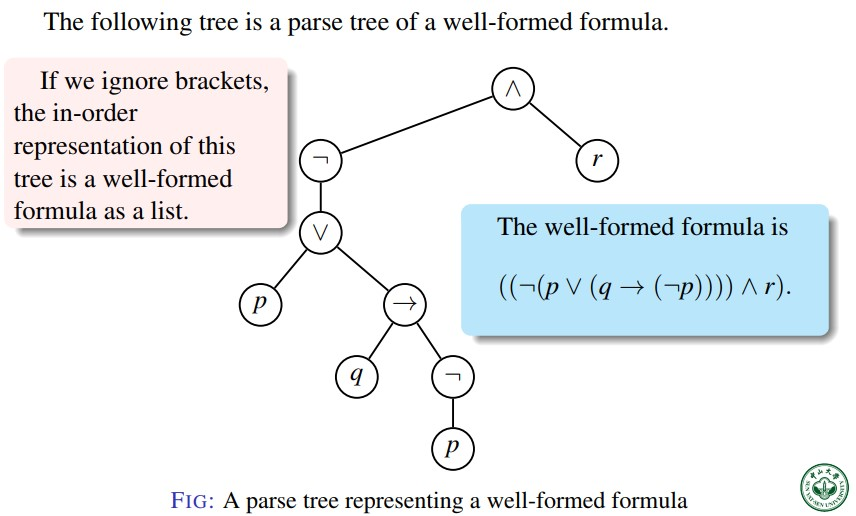
\includegraphics[width=0.8\linewidth]{fig/well-formed_formula.jpg}
\end{figure}
\end{example}

\subsection{语义}
\begin{definition}[模型(model)]
在前提$\phi_1,\phi_2,\ldots,\phi_n$和结论$\psi$上定义另一关系,记作
\[\phi_1,\phi_2,\ldots,\phi_n\models\psi\]
真值包括两个元素$T$和$F$,公式$\phi$的模型(model)或估值(valuation)是指对$\phi$中的每一原子命题都有一个真值指派(assignment)。
对$\phi_1,\phi_2,\ldots,\phi_n$的真值指派决定了$\psi$的真值,称为$\psi$的解释(interpretation),可表示为真值表中的一行。

如果对于所有$\phi_1,\phi_2,\ldots,\phi_n$的估值都为$T$,$\psi$也估值为$T$,那么称
\[\phi_1,\phi_2,\ldots,\phi_n\models\psi\]
成立(hold),且称$\models$为语义后承(semantic entailment)关系。
\end{definition}
\begin{theorem}[可靠性(soundness)]
令$\phi_1,\phi_2,\ldots,\phi_n$和$\psi$都是命题逻辑公式,若$\phi_1,\phi_2,\ldots,\phi_n\vdash\psi$是有效的\footnote{可以由$\phi_1,\ldots,\phi_n$推出$\psi$},那么$\phi_1,\phi_2,\ldots,\phi_n\models\psi$成立。
\end{theorem}
\begin{theorem}[完备性(completeness)]
若$\phi_1,\ldots,\phi_n\models\psi$成立,则存在自然推断证明$\phi_1,\ldots,\phi_n\vdash\psi$。
\end{theorem}
\begin{theorem}
对于命题逻辑来说,完备性和可靠性是等价的。
\end{theorem}

\begin{definition}[恒真式(tautology)/矛盾式(contradiction)]
命题逻辑$\phi$被称为恒真式当且仅当它在所有估值下都取值为$T$,也即$\models\phi$。
若所有估值均为$F$,则为矛盾式。
\end{definition}
\begin{theorem}
若$\models\eta$成立,则$\vdash\eta$是有效的。
换句话说,若$\eta$是永真式,则$\eta$是定理。
\end{theorem}

几个常见逻辑符号的区别\footnote{参考以下资料:
\begin{itemize}
	\item \url{https://math.stackexchange.com/questions/2903877/to-vs-vdash-in-logic}
	\item 逻辑学中,前提为假而命题为真的推论如何解释? - 罗心澄的回答 - 知乎 \url{https://www.zhihu.com/question/21020308/answer/16917222}
	\item 数理逻辑$\implies$,$|$ - 这两个符号有什么区别? - 罗心澄的回答 - 知乎 \url{https://www.zhihu.com/question/21191299/answer/17469774}
	\item 逻辑学蕴涵命题中的$\to$和数学中的$\implies$有什么区别和共同点? - 罗心澄的回答 - 知乎 \url{https://www.zhihu.com/question/276859264/answer/459951353}
\end{itemize}}:
\begin{itemize}
\item \textbf{语义后承}(semantic consequence),符号是$\models$\verb'\models'。
语义后承在一般情况下是连接一个命题集合和一个命题。
如果在任何一种语义赋值$\mM$下,只要命题集合$\Gamma$中的每一个命题都为真(\textbf{真值表}方式),那么$\phi$就一定为真,那么我们就说$\phi$是$\Gamma$的语义后承,记作$\Gamma\models\phi$。
\item \textbf{句法后承}(syntactic consequence),符号是$\vdash$\verb'\vdash'。
句法后承的用法和语义后承类似,也是连接一个命题集合和一个命题,如$\Gamma\vdash\phi$,表示的是$\phi$可以通过\textbf{句法证明}的方式从命题集$\Gamma$中得出。
以Hilbert style的证明为例,这即是说,存在一个命题序列,使得每个前提要么是公理,要么是$\Gamma$中的命题,而这个命题序列的最后一项是$\phi$。
\item \textbf{实质蕴含}(material implication / material conditional),符号是$\to$\verb'\to',当然在强调和不同蕴涵词对比的时候,我们可能会用箭头表示特殊的蕴涵,而用马蹄符号$\supset$表示实质蕴涵,这个取决于作者)。
实质蕴含是一个命题逻辑中的二元算子,连接的是两个命题。
在句法系统中,由Hilbert的前两条公理完全刻画,由第三条公理刻画它和否定的关系。
在语义系统中,我们说$\mM\models\phi\to\psi$当且仅当$\mM\models\psi$或者$\mM\not\models\phi$。
\end{itemize}
可以理解为$\vdash$左侧是一些公理(axiom),右侧是陈述(statement);而$\to$只是一个连接符,本身并不包含推理的信息。
$p\to q$更像是一个数字(如$2+2$),而不是一个判断,它只表达了纯粹的命题内容。
要断定它,更应该说“$p\to q$为真”才行。

\subsection{范式}
\begin{definition}[语义等价]
$\phi$和$\psi$都是命题逻辑的公式,称其等价当且仅当$\phi\models\psi$和$\psi\models\phi$成立,记作$\phi\equiv\psi$,也等价于$\models(\phi\to\psi)\land(\psi\to\phi)$成立。
\end{definition}
\begin{definition}[合取范式(conjunction normal form, CNF)]
BNF定义如下:
\begin{itemize}
	\item 文字(literal):$L::=p\mid\lnot p$
	\item 句子(clause):$D::=L\mid L\lor D$
	\item 公式(formula):$C::=D\mid(D)\mid D\land C$
\end{itemize}
例子如
\[(p \lor r) \land (\lnot p \lor r) \land (p \lor \lnot r)\]
\end{definition}
\begin{definition}[可满足的(satisfiable)]
令$\phi$为命题逻辑公式,$\phi$是可满足的当且仅当$\lnot\phi$不是有效的。
\end{definition}

\begin{definition}[霍尔公式(Horn formula)]
若命题逻辑公式$\phi$能用下面的语法,表示成$H$的一个示例
\[P::=\bot\mid\top\mid p\qquad
A::=P\mid P\land A
C::=A\to P
H::=C\mid C\land H\]
则称$C$的每个实例为霍尔从句(clause)。
\end{definition}

\subsection{SAT求解器}
线性求解器只接受以下几种形式的公式
\[\phi::=p\mid(\lnot\phi)\mid(\phi\land\phi)\]
\begin{example}
$\phi=p\land\lnot(q\lor\lnot p)$,计算$T(\phi)=p\land\lnot\lnot(\lnot q\land\lnot\lnot p)$,则有语法树和DAG如下
\begin{figure}[H]
\centering
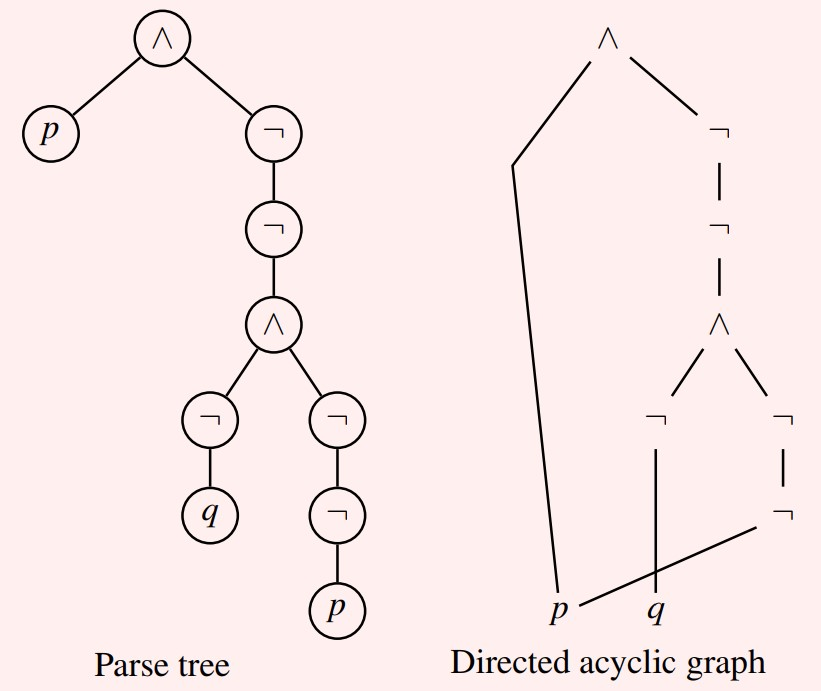
\includegraphics[width=0.5\linewidth]{fig/parse_tree_dag_eg.jpg}
\end{figure}
\end{example}